 \documentclass{article}
\usepackage[francais]{babel}
\def\printlandscape{\special{landscape}}    
\usepackage{amsmath}
\usepackage[utf8]{inputenc}
\usepackage[T1]{fontenc} 
\usepackage{fancybox} 
\usepackage{alltt}
\usepackage{graphicx}
\usepackage{lmodern}
\usepackage[colorlinks,hyperindex,bookmarks,linkcolor=blue,citecolor=blue,urlcolor=blue]{hyperref}
\usepackage{epsf}
\usepackage{enumitem}
\usepackage{pifont}
\usepackage{hyperref}
\usepackage{authblk}
\usepackage{titling}
\usepackage{floatflt}
\usepackage{changepage}
\usepackage[margin=0.5in]{geometry}
\usepackage{parskip}
\usepackage{subfig}
\setlength{\parindent}{30pt}

\begin{document}
\begin{center}
{\huge \textbf{Rapport de Début de Projet}}
\end{center}

\begin{center}
Participants : \textit{Baudet Léo-Paul / Miniaou Lucie / Tournier Pauline / Nguyen Mathieu\\}

\end{center}
\vspace{0.05\textheight}
\begin{center}
{\LARGE \textbf{Contrôle Magnétique d'Interface Liquides}}
\end{center}

\section{Travail de Mathieu et Léo-Paul}
Léo-Paul s'est assuré dans un premier temps que les différentes méthodes de résolution numérique étaient applicables sur notre équation, notamment la méthode de Nexton. Pour cette méthode, il faut vérifier que la dérivée ne s'annule pas, peu importe le x. Une fois que cela est fait, il a pu implémenter toutes les méthodes de résolution, à savoir \textbf{la dichotomie, le point fixe de Picard et la méthode de Newton}.
\newline
Mathieu a commencé par implémenter les différents champs que l'on peut retrouver dans notre situation, plus spécialement les champs qui admettent \textbf{une invariance en y} (afin de n'avoir que x et z comme inconnues). On s'est finalement penché sur les 3 cas suivant : la nappe de courant, les deux fils à courant inversé et le dipole magnétique.
\newline
La nappe de courant est le champ le plus simple à mettre en place, car si on envoie le courant selon Oy, alors on n'a un \textbf{champ qui ne dépend que de z}. L'équation implémenté est la suivante : 

\begin{equation}
H(M) = \frac{jS}{2}\vec{u_{z}}
\label{eq08}
\end{equation}
\begin{figure}[h]
	\centering
    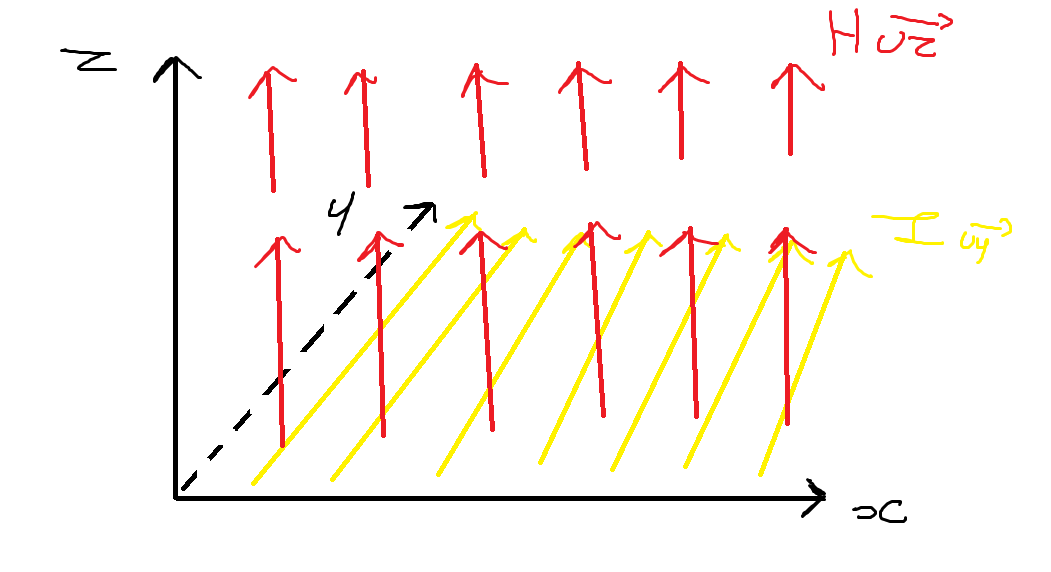
\includegraphics[width=.5\linewidth]{Nappe.png}
    
\end{figure}

Les deux fils à courant sont plus complexes à définir, car leur champ est la plupart du temps donné dans des coordonnées cylindriques, et nous voulons les implémenter en coordonnées cartésiennes. Encore une fois, on fait en sorte d'avoir une \textbf{invariance en y}. Cela nous donne les formules suivantes :

\begin{equation}
H_{x}=\frac{-1}{\pi}pI\frac{2xz}{(x^2-y^2-p^2)^2+4x^2y^2} \indent\indent  H_{z}=\frac{-1}{\pi}pI\frac{x^2-y^2-p^2}{(x^2-y^2-p^2)^2+4x^2y^2}
\label{eq09}
\end{equation}
\begin{equation}
p = \sqrt{\frac{d^2}{4} - r^2} \indent\indent |H| = \sqrt{H_{x}^2+H_{z}^2}
\label{eq10}
\end{equation}
\begin{figure}[h]
	\centering
    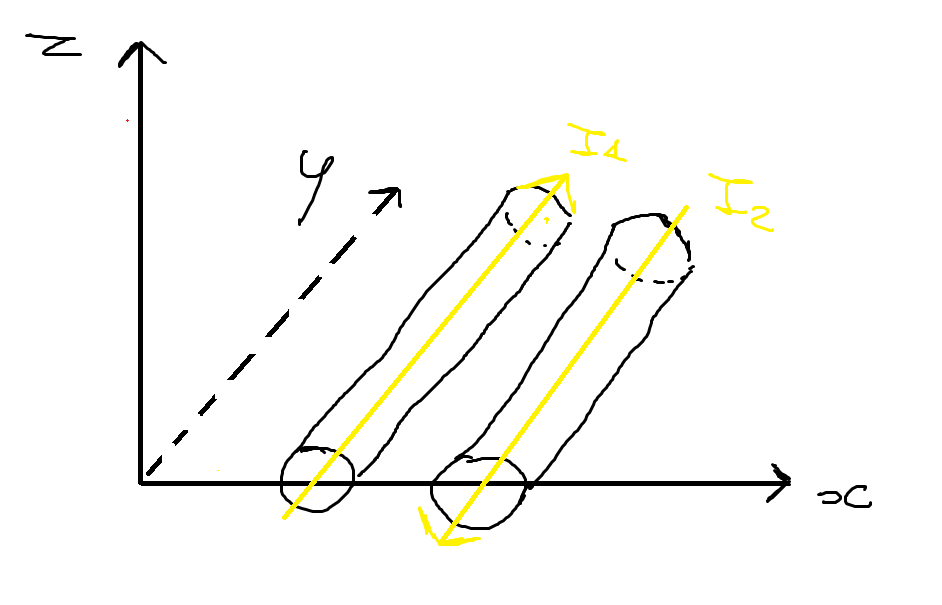
\includegraphics[width=.4\linewidth]{Fils.png}
    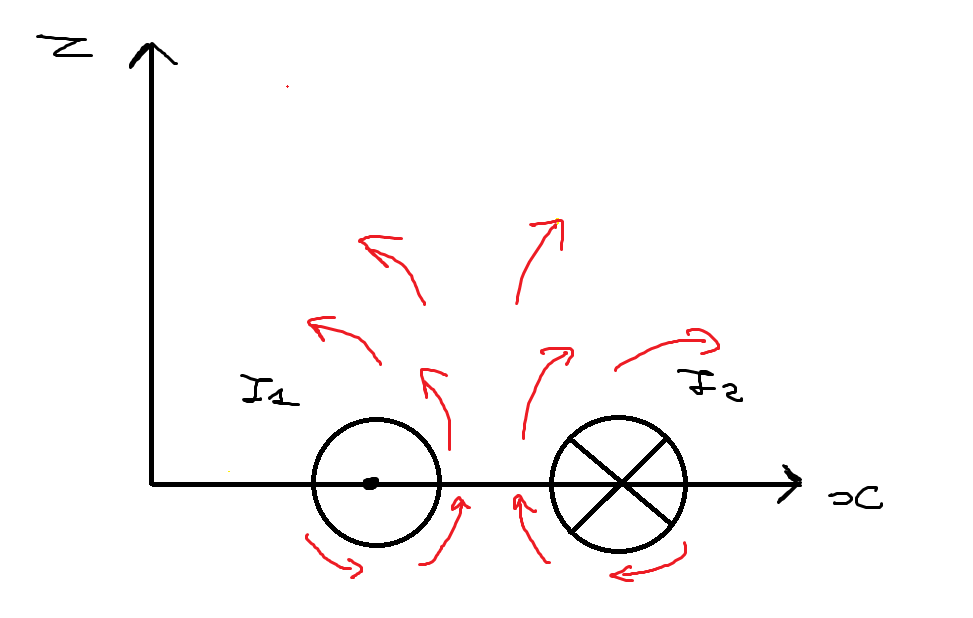
\includegraphics[width=.4\linewidth]{Fils2.png}
\end{figure}

Pour implémenter le dipôle magnétique, j'utilise la formule en carthésien suivante en considérant $m = IS$ :
\begin{equation}
H_{x} = \frac{m}{4\pi}\frac{3zx}{r^5}\indent\indent H_{y} = \frac{m}{4\pi}\frac{3zy}{r^5}\indent\indent H_{z}=\frac{m}{4\pi}\frac{1}{r^3}[\frac{3z^2}{r^2} - 1]
\end{equation}
En rappelant \textbf{$r = \sqrt{x^2 + y^2 +z^2}$}
\begin{figure}[h]
	\centering
    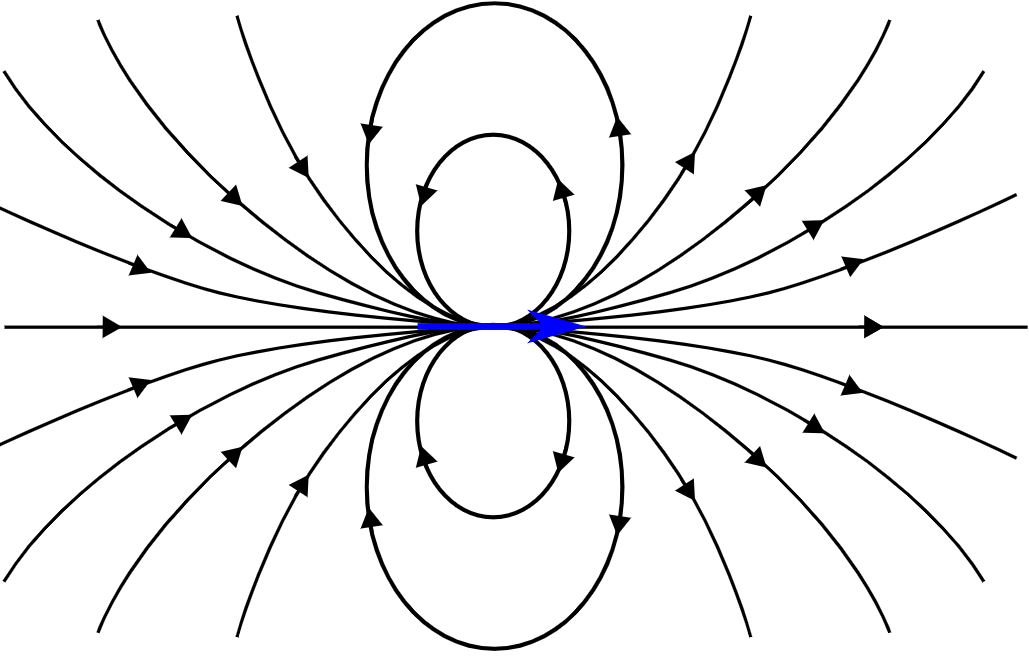
\includegraphics[width=.5\linewidth]{Dipole.png}
    
\end{figure}
\end{document}
   